%\documentclass[a4paper]{jarticle}

\documentclass[letterpaper]{article}

\usepackage{tabularx}
\usepackage{color}
%\usepackage{doublespace}
%\setstretch{1.2}
\usepackage{graphicx}

\usepackage{ae}
\usepackage[T1]{fontenc}
\usepackage{CV}

\usepackage{fullpage}
%\setlength{\textwidth}{\fullwidth}

\begin{document}

\pagestyle{empty}

%Ueberschrift
\begin{center}
  \huge{\textsc{Curriculum Vitae}}
%\huge{\textsc{履歴書}}
\vspace{\baselineskip}

\Large{\textsc{Dr. Ryoji Tanabe}}
\end{center}
\vspace{1.5\baselineskip}


\section{}

 \begin{flushright}
   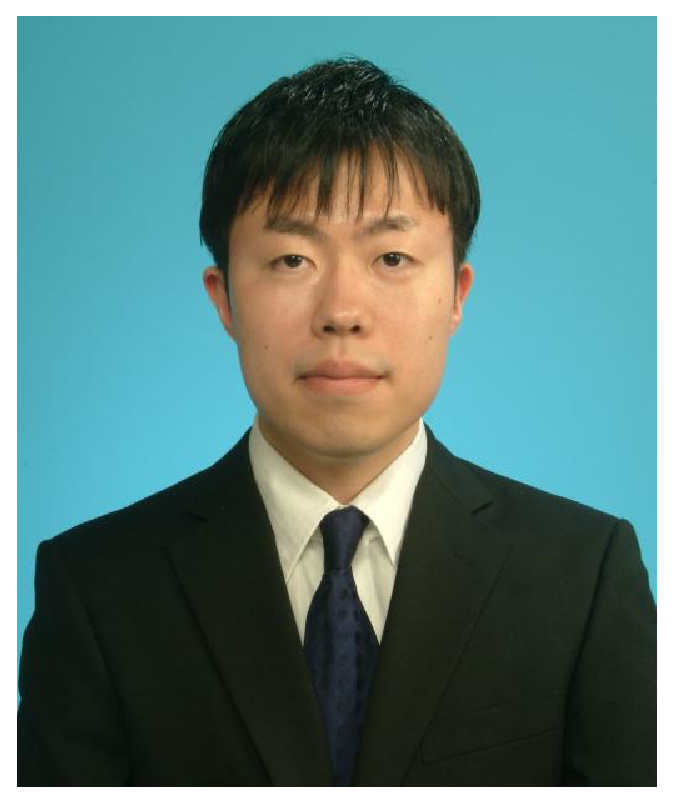
\includegraphics[width=.2\linewidth]{tanabe.eps}
 \end{flushright}

\section{\textcolor{blue}{Personal Details}}

\begin{flushleft}
Affiliation: Institute of Space and Astronautical Science, Japan Aerospace Exploration Agency (ISAS/JAXA)\\
%  住所: 153-8902 東京都目黒区駒場 3-8-1\\
Address: 3-1-1 Yoshinodai, Chuo-ku, Sagamihara City, Kanagawa Prefecture, 252-5210\\
%  住所: 206-0011 東京都多摩市関戸1-1-5ザ$\cdot$スクエアC629\\
Date of birth: 7th of December, 1987\\
Present Citizenship: Japan\\
%  生年月日: 1987年12月7日 (満27歳)\\
  %% Steenhouwerskade 12345 \\
  %% 9718 DL G-Town \\
  %% The Netherlands \\
%  Fax: +31-50-363.7337 \\
  Email: rt.ryoji.tanabe@gmail.com or tanabe@flab.isas.jaxa.jp\\
  Phone: +81-90-5785-6784 \\
  Homepage: https://sites.google.com/site/tanaberyoji/
\end{flushleft}


%% \section{Personal Details}
%% \begin{flushleft}
%%     %% Gender: Male \\
%%   %% Date of birth: 36th of November, 1971 \\
%%   %% Place of birth: R-Town, Germany \\
%%   %% Present Citizenship: German
%% \end{flushleft}

%\pagebreak

%% \section{Thesis}
%% \noindent A special feature of the German financial system is the position of
%% the \emph{Deutsche Bundesbank}, which is considered to be one of the
%% most independent central banks in the world. The purpose of this
%% research is to analyse to which extent this formal independent
%% position has led to less political influence on the central
%% bank than, for instance, in the USA.


\section{\textcolor{blue}{Research Interests}}

\begin{itemize}
  \item Computational Intelligence
  \item Evolutionary Computation
  \item Single/Multi-Objective Continuous Optimization   
\end{itemize}


\clearpage


\section{\textcolor{blue}{Education}}

\begin{CV}
\item[March, 2016] Ph.D. degree in Science from The University of Tokyo
\item[March, 2013] MS degree in Engineering from Sophia University
\item[March, 2011] BS degree in Engineering from Sophia University
\end{CV}


\section{\textcolor{blue}{Work Experience}}

\begin{CV}
\item[April 2014 $\sim$ March 2016] Research Fellow of Japan Society for the Promotion of Science (DC2)
\item[April 2016 $\sim$] Postdoctoral researcher at Institute of Space and Astronautical Science, Japan Aerospace Exploration Agency (ISAS/JAXA)
\end{CV}



\section{\textcolor{blue}{Awards}}

\begin{enumerate}
\item Winner of the IEEE CEC2014 Competition on Real-Parameter Single Objective Optimization 
\item ACM GECCO Student Travel Award, 2014.
\item IEEE CIS Outstanding Student-Paper Travel Grant Award, 2014.
\item IEEE CIS Outstanding Student-Paper Travel Grant Award, 2013.
\end{enumerate}


\section{\textcolor{blue}{Professional Activities/Service}}
\begin{itemize}
\item Reviewer of Journals
\begin{itemize}
\item IEEE Transactions on Evolutionary Computation
\item IEEE Transactions on Cybernetics
\item IEEE Transactions on Fuzzy Systems
\item IEEE Access
\item Swarm and Evolutionary Computation
\item Memetic Computing
\item Applied Soft Computing
\item Information Processing Letters
\end{itemize}
\item Conference Program Committee member
\begin{itemize}
\item GECCO: 2016, 2017
\item CEC: 2014, 2016
\end{itemize}
\end{itemize}


%% \section{Language Knowledge}
%% \begin{table}[h] %\centering
%% \begin{tabular}{p{2cm}>{\bfseries}p{2.5cm}p{3cm}}
%% & German  & native \\
%% & French  & near native \\
%% & Dutch & near native\\
%% & Italian & fair \\
%% \end{tabular}
%% \end{table}

\clearpage

\section{\textcolor{blue}{Publication}}

{\bf Peer Reviewed Conference Papers}
\begin{enumerate}
\small
\item \underline{Ryoji Tanabe} and Akira Oyama: \\\textcolor{blue}{The Impact of Population Size, Number of Children, and Number of Reference Points on The Performance of NSGA-III}, \\Proc. Evolutionary Multi-Criterion Optimization ({\bf EMO-2017}), M\"unster, March, 2017 (accepted)
\item \underline{Ryoji Tanabe} and Alex Fukunaga: \\\textcolor{blue}{How Far Are We From an Optimal, Adaptive DE?}, \\Proc. Parallel Problem Solving from Nature ({\bf PPSN-2016}), pp. 145-155, Edinburgh, September, 2016
\item \underline{Ryoji Tanabe}: \\\textcolor{blue}{A Note on Multi-Funnel Functions for Expensive Optimization Scenario}, \\Proc. Genetic and Evolutionary Computation Conference ({\bf GECCO-2015}, poster), pp. 1493-1494, Madrid, July, 2015
\item \underline{Ryoji Tanabe} and Alex Fukunaga: \\\textcolor{blue}{Tuning Differential Evolution for Cheap, Medium, and Expensive Computational Budgets},\\ Proc. IEEE Congress on Evolutionary Computation ({\bf CEC-2015}), pp. 2018-2025, Sendai, May, 2015
\item Claus de Castro Aranha, \underline{Ryoji Tanabe}, Romain Chassagne, Alex Fukunaga: \\\textcolor{blue}{Optimization of Oil Reservoir Models Using Tuned Evolutionary Algorithms and Adaptive Differential Evolution}, \\Proc. IEEE Congress on Evolutionary Computation ({\bf CEC-2015}), pp. 877-884, Sendai, May, 2015
%
\item \underline{Ryoji Tanabe} and Alex Fukunaga: \\\textcolor{blue}{Reevaluating Exponential Crossover in Differential Evolution}, \\Proc. Parallel Problem Solving from Nature ({\bf PPSN-2014}), pp. 201-210, Ljubljana, September, 2014
\item \underline{Ryoji Tanabe} and Alex Fukunaga:\\ \textcolor{blue}{On the Pathological Behavior of Adaptive Differential Evolution on Hybrid Objective Functions},\\ Proc. ACM Genetic and Evolutionary Computation Conference ({\bf GECCO-2014}), pp. 1335-1342, Vancouver, July, 2014
\item \underline{Ryoji Tanabe} and Alex Fukunaga: \\\textcolor{blue}{Improving the Search Performance of SHADE Using Linear Population Size Reduction},\\ Proc. IEEE Congress on Evolutionary Computation ({\bf CEC-2014}),  pp. 1658-1665, Beijing, July, 2014
\item \underline{Ryoji Tanabe} and Alex Fukunaga:\\ \textcolor{blue}{Evaluation of a Randomized Parameter Setting Strategy for Island-Model Evolutionary Algorithms}, \\Proc. IEEE Congress on Evolutionary Computation ({\bf CEC-2013}), pp. 1263-1270, Cancun, June, 2013
\item \underline{Ryoji Tanabe} and Alex Fukunaga:\\ \textcolor{blue}{Success-History Based Parameter Adaptation for Differential Evolution}, \\Proc. IEEE Congress on Evolutionary Computation ({\bf CEC-2013}), pp. 71-78, Cancun, June, 2013
\item \underline{Ryoji Tanabe} and Alex Fukunaga:\\ \textcolor{blue}{Evaluating the performance of SHADE on CEC 2013 benchmark problems}, \\Proc. IEEE Congress on Evolutionary Computation ({\bf CEC-2013}), pp. 1952-1959, Cancun, June, 2013.
\end{enumerate}

%\clearpage

%\pagebreak

%% \section{\textcolor{blue}{References}}

%% \noindent These persons are familiar with my professional qualifications and my character:

%% \begin{table}[h]
%% \begin{tabular}{@{}lll@{}}
%% \textbf{Prof. Alex Fukunaga} \\
%% Thesis supervisor & Phone: & +31-50-312.3456\\
%% P.O. Box 800 & Fax: & +31-50-567.123\\
%% 9700 AV Groningen & Email: & p.fessor@xxx.rug.nl \\
%% The Netherlands \\
%% \end{tabular}
%% \end{table}

%% \vspace{2\baselineskip}
%% \noindent Groningen, \today



\end{document}

%Tabellen
\begin{table}[htbp] \centering%
\begin{tabular}{lll}\hline\hline
1 & 2 & 3 \\ \hline
1 & \multicolumn{2}{c}{2} \\
\hline
\end{tabular}
\caption{Titel\label{Tabelle: Label}}
\end{table}






